\documentclass[11pt]{article}
\usepackage[margin=1in]{geometry}
\usepackage{amsmath,amssymb}
\usepackage{booktabs,graphicx,float,caption}
\usepackage[colorlinks=true,urlcolor=blue]{hyperref}

\newcommand{\R}{\mathbb{R}}

\title{DATA 37711 --- Homework 2}
\author{Hetav Mehta}
\date{November 6, 2025}

\begin{document}
\maketitle

\begin{center}
Code: \url{https://github.com/HetavMehta999/STAT-37711-Homework/tree/main/homework_2}
\end{center}

%==============================================================================
\section*{Problem 1}
%==============================================================================

\subsection*{(a)}
Write $g(x) = (g_1(x), g_2(x))$. The mean is unconstrained and the standard deviation must be positive, so we use
\[
  f_\mu(x) = g_1(x), \qquad f_\sigma(x) = \operatorname{softplus}(g_2(x)) + \varepsilon = \log\!\bigl(1+e^{g_2(x)}\bigr) + \varepsilon,
\]
with a small $\varepsilon>0$ for numerical stability. $f_\sigma(x)=\exp(g_2(x))$ also works. Softplus grows only linearly in $g_2$, which keeps gradients stable.

\subsection*{(b)}
We use the negative log-likelihood of $Y\mid X \sim \mathcal N(f_\mu(X), f_\sigma(X)^2)$:
\[
  \mathcal L(\theta) = \frac1n\sum_{i=1}^n \left[ \log f_\sigma(x_i) + \frac{\bigl(y_i - f_\mu(x_i)\bigr)^2}{2 f_\sigma(x_i)^2} \right] + \text{const}.
\]
With a constant $f_\sigma$ this reduces to mean squared error. When $f_\sigma$ is allowed to vary, errors on inherently noisy inputs are down-weighted, and the $\log f_\sigma$ term stops the model from inflating $\sigma$ everywhere.

\subsection*{(c)}
\textbf{Setup.} There are 523{,}554 trips. We use a seeded random 70/15/15 train/validation/test split and standardize the target with training-set statistics. The model is an MLP
$7\to256\to256\to128\to2$ with SiLU activations and the link from (a). We train it on the NLL from (b) with AdamW (lr $10^{-3}$, batch size 1024), reduce the learning rate on plateau, and stop early
on validation NLL.

\textbf{Baselines,} all trained on the same split: (i) a constant Gaussian $\mathcal N(\bar y, s_y^2)$; (ii) a linear model for both $f_\mu$ and $g_2$, trained on the same NLL;
(iii) the same MLP with a single constant $\sigma$, which isolates the benefit of modeling $f_\sigma(x)$; and, for part (e), (iv) a constant probability equal to the training base rate.

\begin{table}[H]
\centering\small
\begin{tabular}{lccc|ccc}
\toprule
 & \multicolumn{3}{c|}{Regression, part (c)} & \multicolumn{3}{c}{$P(\text{trip}<45\text{ min})$, part (e)} \\
Model & NLL & RMSE & MAE & Brier & Log-loss & Accuracy \\
\midrule
Constant base rate & -- & -- & -- & 0.00444 & 0.0286 & 0.9955 \\
Constant Gaussian & 3.466 & 7.75 & 5.70 & 0.00446 & 0.0552 & 0.9955 \\
Linear (heterosc.) & 3.405 & 7.61 & 5.60 & 0.00444 & 0.0421 & 0.9955 \\
MLP, constant $\sigma$ & 2.714 & 3.65 & 2.31 & 0.00282 & 0.0253 & 0.9968 \\
\textbf{MLP, $f_\mu$ and $f_\sigma$} & 2.622 & 3.77 & 2.40 & 0.00291 & 0.0177 & 0.9967 \\
\bottomrule
\end{tabular}

\caption*{Test-set results. NLL is per trip, with $y$ in minutes.}
\end{table}

\noindent Both MLPs beat the constant and linear baselines by a wide margin, with RMSE falling from about 7.7 to about 3.7 minutes. Trip duration depends nonlinearly on
the pickup and dropoff coordinates. The MLP with $f_\sigma(x)$ has the best test NLL (2.62 vs.\ 2.71), so it gives the best predictive distribution. Its
RMSE is slightly higher than the constant-$\sigma$ MLP's (3.77 vs.\ 3.65) because the NLL down-weights trips it predicts to be noisy. The right panel below shows that
$f_\sigma$ is well calibrated: the observed residual spread tracks the predicted $\sigma$.

\begin{figure}[H]
  \centering
  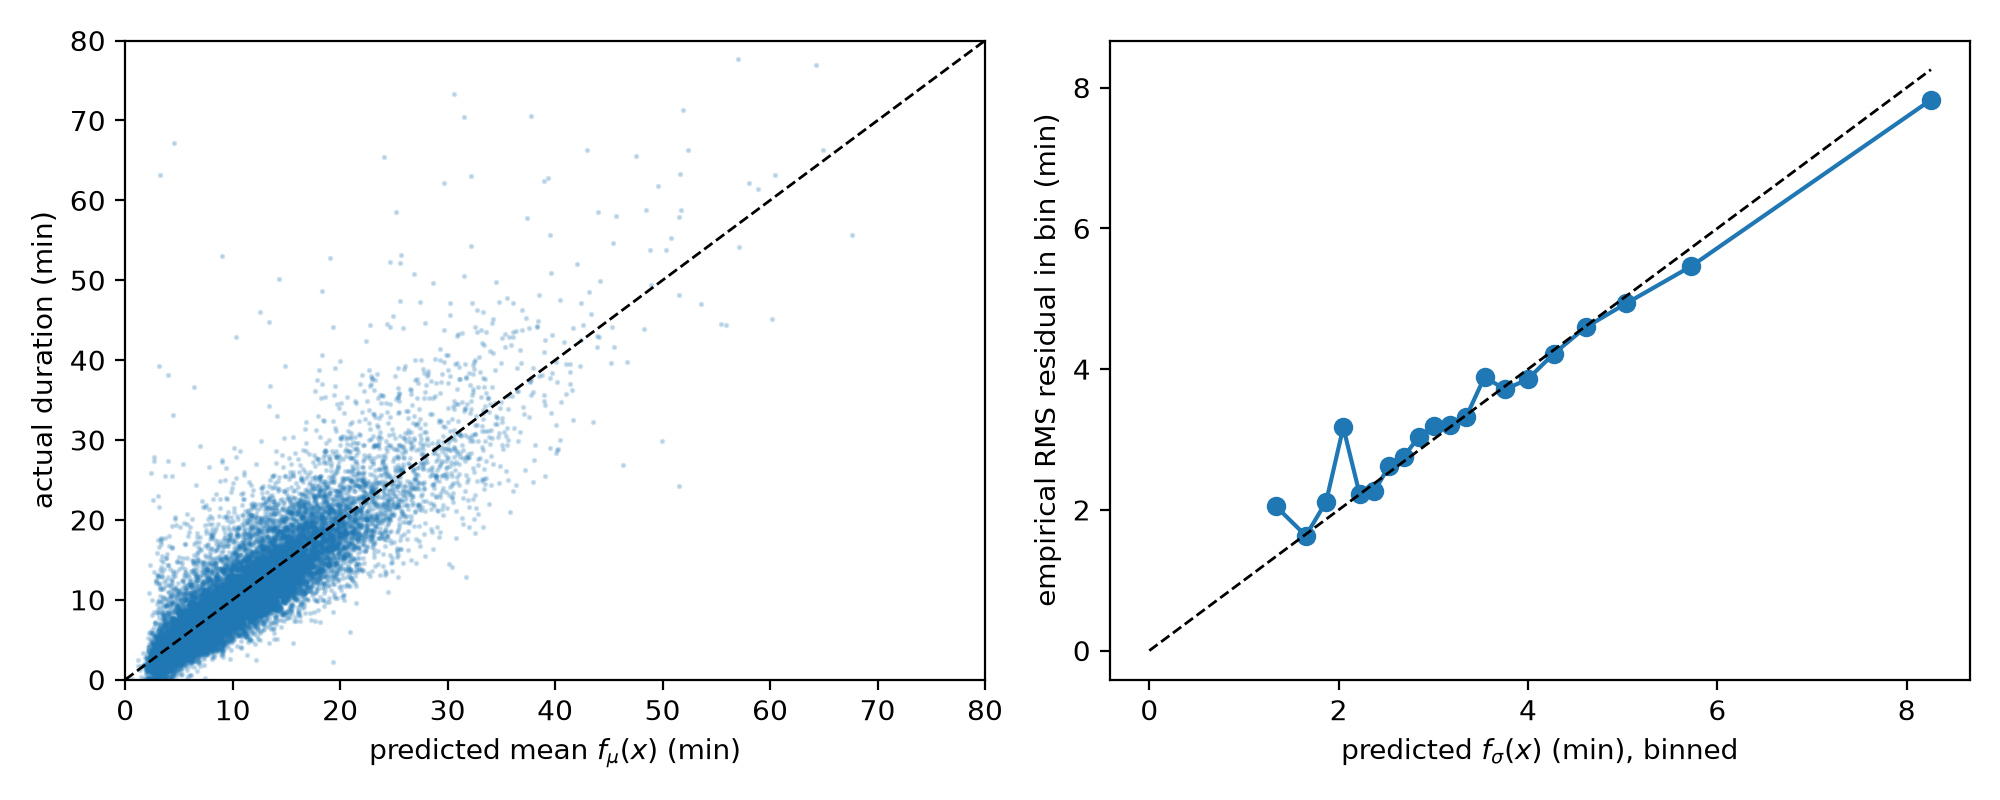
\includegraphics[width=\linewidth]{../problem1/results/mean_and_sigma_fit.png}
  \caption{Test set. Left: predicted mean vs.\ actual duration. Right: predicted $f_\sigma(x)$ (20 quantile bins) vs.\ RMS residual in each bin.}
\end{figure}

\subsection*{(d)}
Under the fitted model,
\[
  \hat p(x) = P(Y < 45 \mid X=x) = \Phi\!\left(\frac{45 - f_\mu(x)}{f_\sigma(x)}\right),
\]
where $\Phi$ is the standard normal CDF. Thresholding at $\hat p\ge0.5$ is equivalent to $f_\mu(x)\le45$, but the probability itself depends on $f_\sigma(x)$.

\subsection*{(e)}
The right half of the table above reports the Brier score and log-loss of $\hat p$ (both proper scoring rules, lower is better) and the accuracy at threshold 0.5.
Since 99.55\% of test trips are under 45 minutes, the base-rate predictor already reaches 99.55\% accuracy, so that is the bar to beat. The MLP with $f_\sigma(x)$
achieves Brier $0.00291$, log-loss $0.0177$ and accuracy $99.67\%$. That is a 34\% lower Brier score, a 38\% lower log-loss, and about a quarter fewer errors than the base rate.
Compared with the constant-$\sigma$ MLP, accuracy and Brier score are similar, but log-loss is much better ($0.0177$ vs.\ $0.0253$). A constant $\sigma$ is too small for long,
uncertain trips, which produces confident mistakes that the log-loss penalizes heavily.

%==============================================================================
\section*{Problem 2}
%==============================================================================
\texttt{Quantity} is extremely heavy-tailed (median 6, maximum 80{,}995), so every model is trained with squared error on $y=\log(1+\texttt{Quantity})$,
i.e.\ a log-normal model. We report errors on the log scale, plus MAE in units of \texttt{Quantity} using $\exp(\hat y)-1$.

\subsection*{(a)}
\texttt{StockCode} has 3{,}665 unique values and \texttt{CustomerID} has 4{,}339, across 397{,}924 rows. The category counts are long-tailed: 472 products and 228 customers
have fewer than 5 rows. One-hot encoding gives 8{,}004 columns. As a dense matrix that is about 12.7\,GB, which is infeasible as input to a neural network. It is feasible only as a sparse matrix for a linear
model, which we fit as a baseline (one-hot + ridge). Even then, every category gets an independent parameter, nothing is shared between similar categories, and
customer$\times$product interactions would need about 15.9M columns. This points to low-dimensional encodings: target encoding or learned embeddings.
We use a seeded random 70/15/15 train/validation/test split. The validation set is used for early stopping and tuning.

\subsection*{(b)}
Each category is replaced by the smoothed mean of $y$ over its training rows, using \texttt{TargetEncoder} from \texttt{category\_encoders}. Training rows are encoded out-of-fold (5-fold), so
a row's encoding never uses its own label. The model is gradient-boosted trees on the two encoded features, trained with squared error on $y$ and with the number of trees chosen on validation.

\subsection*{(c)}
Each feature has its own embedding table of dimension 16, with an extra index for unseen categories. The two embeddings are concatenated and passed through an MLP
$32\to128\to64\to1$ (ReLU, dropout 0.1). We train with AdamW on squared error on $y$, with early stopping on validation. Dimension 16 is small compared with the
thousands of categories but large enough to represent several latent types of product or customer.

\subsection*{(d)}
This is the same network as in (c), with the two target-encoded features concatenated to the embeddings.

\begin{table}[H]
\centering\small
\begin{tabular}{lcccc}
\toprule
Model & RMSE (log) & MAE (log) & $R^2$ (log) & MAE (units) \\
\midrule
Global mean & 1.0011 & 0.8148 & 0.000 & 10.37 \\
One-hot + ridge & 0.5521 & 0.4041 & 0.696 & 6.42 \\
(b) Target encoding + GBM & 0.5834 & 0.4256 & 0.660 & 6.82 \\
(c) Embedding NN & 0.5350 & 0.3829 & 0.714 & 6.26 \\
(d) Embedding + TE NN & 0.5236 & 0.3670 & 0.726 & 6.11 \\
\bottomrule
\end{tabular}

\caption*{Test-set results.}
\end{table}

\noindent Target encoding (b) is a large improvement over the global mean ($R^2=0.66$), but it is worse than one-hot ridge. Target encoding uses each feature's \emph{marginal} mean, so a
product bought mostly by wholesalers looks like a high-quantity product regardless of who is buying it. Ridge estimates the product and customer effects jointly.
The embedding network (c) beats both (RMSE 0.535 vs.\ 0.583 for (b), MAE 6.26 vs.\ 6.82 units). Combining embeddings with target encoding (d) is best (RMSE 0.524,
$R^2=0.726$). That is a 2\% gain over (c) and 10\% over (b), so the embeddings already capture most of what the target encodings carry.

\subsection*{(e)}
An embedding layer is a learned lookup table. It is equivalent to a one-hot encoding followed by a low-rank linear layer $W\in\R^{K\times16}$. Each product and
customer becomes a point in $\R^{16}$, learned to predict quantity. Because $16\ll K$, categories have to share directions, so similar products and similar customers (for example,
bulk vs.\ gift items, wholesale vs.\ retail buyers) end up close together. As in collaborative filtering, a customer--product pair that was never observed is predicted from
how similar customers bought similar products. Only 0.27M of the 15.9M possible pairs ever occur. The MLP on top can also model \emph{interactions}: the same product is bought
singly by one customer and by the dozen by another. Neither an additive model nor a single marginal mean per category can express that.

\begin{table}[H]
\centering\small
\resizebox{\linewidth}{!}{\begin{tabular}{lccccc}
\toprule
Training rows of rarer category & unseen (0) & 1-9 & 10-49 & 50-199 & 200+ \\
Share of test rows & 0.001 & 0.032 & 0.264 & 0.527 & 0.175 \\
\midrule
Global mean & 1.381 & 1.116 & 0.992 & 0.975 & 1.065 \\
One-hot + ridge & 1.002 & 0.588 & 0.534 & 0.538 & 0.606 \\
(b) Target encoding + GBM & 1.017 & 0.785 & 0.592 & 0.554 & 0.607 \\
(c) Embedding NN & 1.058 & 0.592 & 0.521 & 0.520 & 0.582 \\
(d) Embedding + TE NN & 1.076 & 0.601 & 0.515 & 0.505 & 0.568 \\
\bottomrule
\end{tabular}
}
\caption*{Test RMSE (log scale) by number of training rows of the row's rarer category (customer or product).}
\end{table}

\noindent The test set supports this. For rare categories (1--9 training rows), target encoding is much worse (0.785) than the embedding network (0.593), because it has to
shrink those categories toward the global mean, while the jointly trained network still learns from the other, better-known feature. For well-populated categories (50+ rows,
70\% of the test set), the embedding models are best (0.505--0.582 vs.\ 0.538--0.607 for ridge and target encoding), which is where interactions can be learned. For
the roughly 70 test rows with an unseen category, all models are poor.

%==============================================================================
\section*{Problem 3}
%==============================================================================

\subsection*{(a)}
\begin{figure}[H]
  \centering
  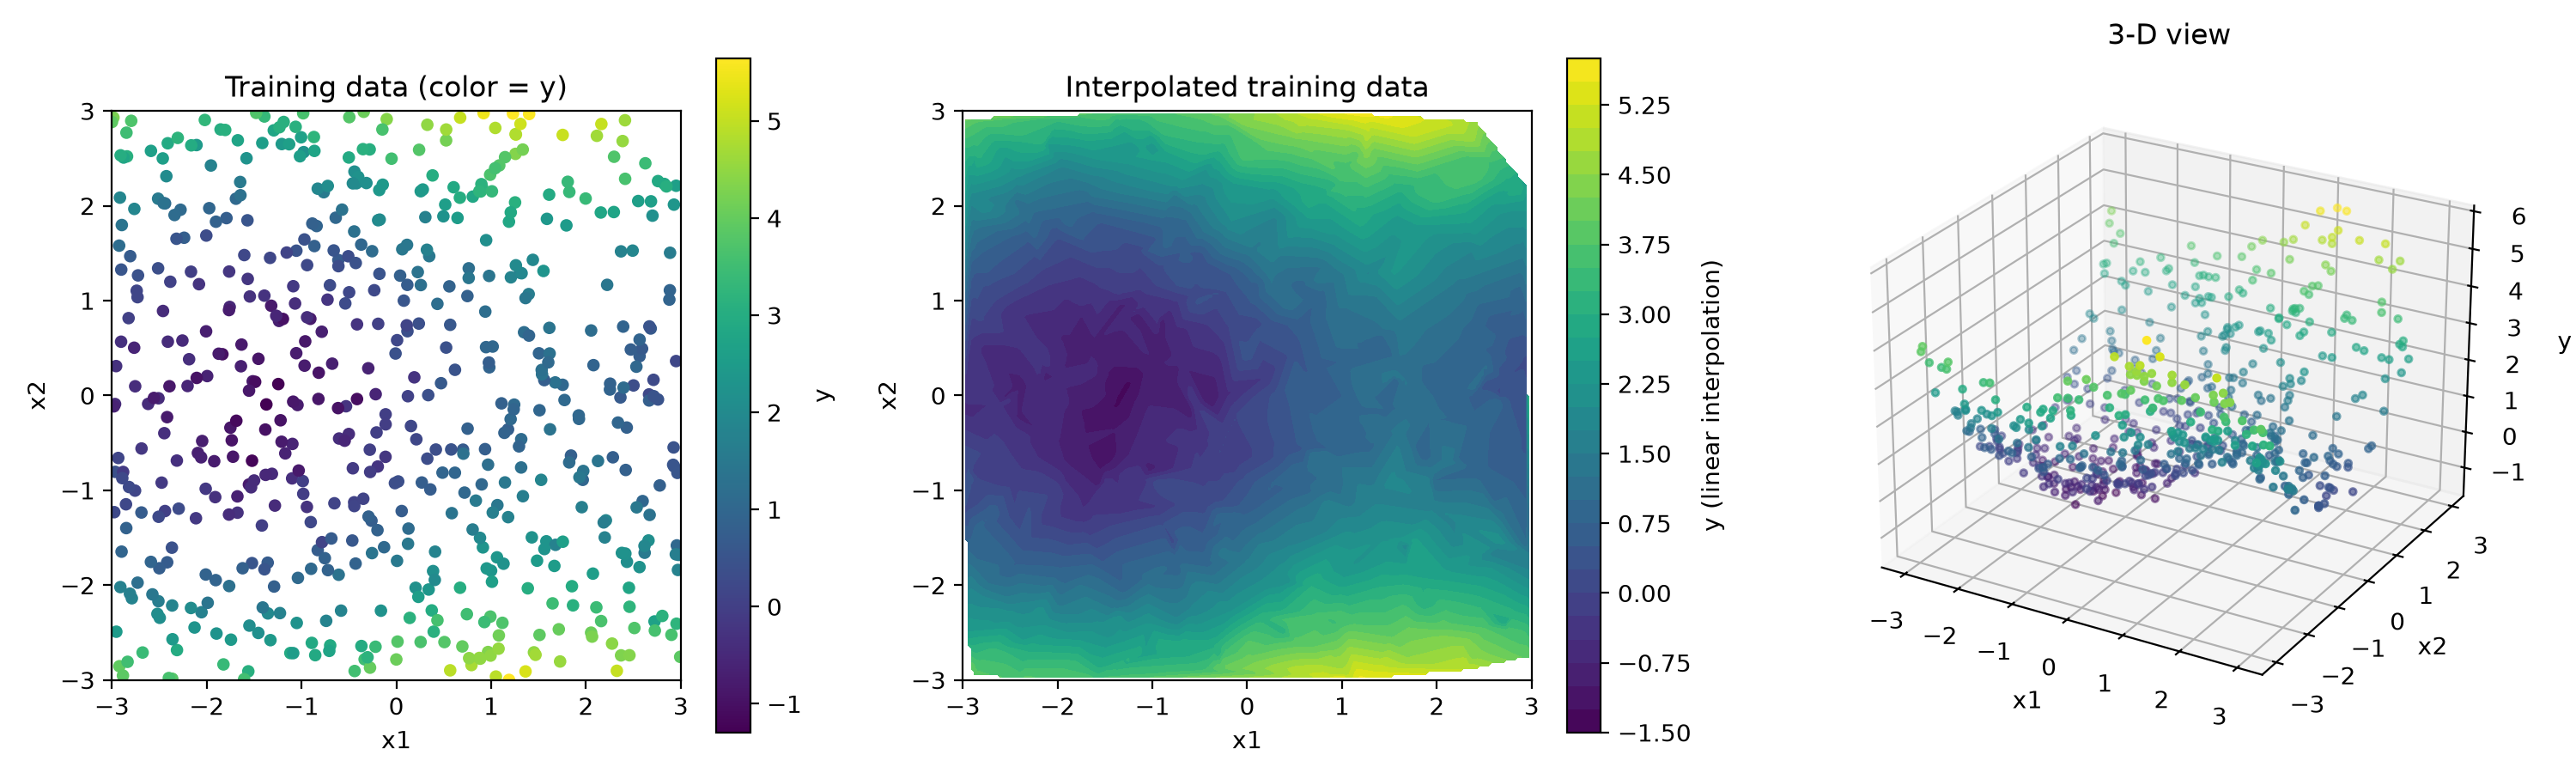
\includegraphics[width=\linewidth]{../problem3/results/training_data.png}
  \caption{Training data: points colored by $y$, linear interpolation, and 3-D view.}
\end{figure}
\noindent The response is a smooth, low-frequency surface with mild noise. It has a basin ($y\approx-1$) near $(-1.5,0)$, a saddle near $(1.5,0)$, and it rises toward
$x_2=\pm3$, peaking at $y\approx5.5$ near $(1.5,\pm3)$.

\subsection*{(b)}
RKS with $D=1000$ features and ridge $\lambda=10^{-3}$ (intercept unpenalized, closed-form fit), sweeping the kernel scale $\sigma$:

\begin{figure}[H]
  \centering
  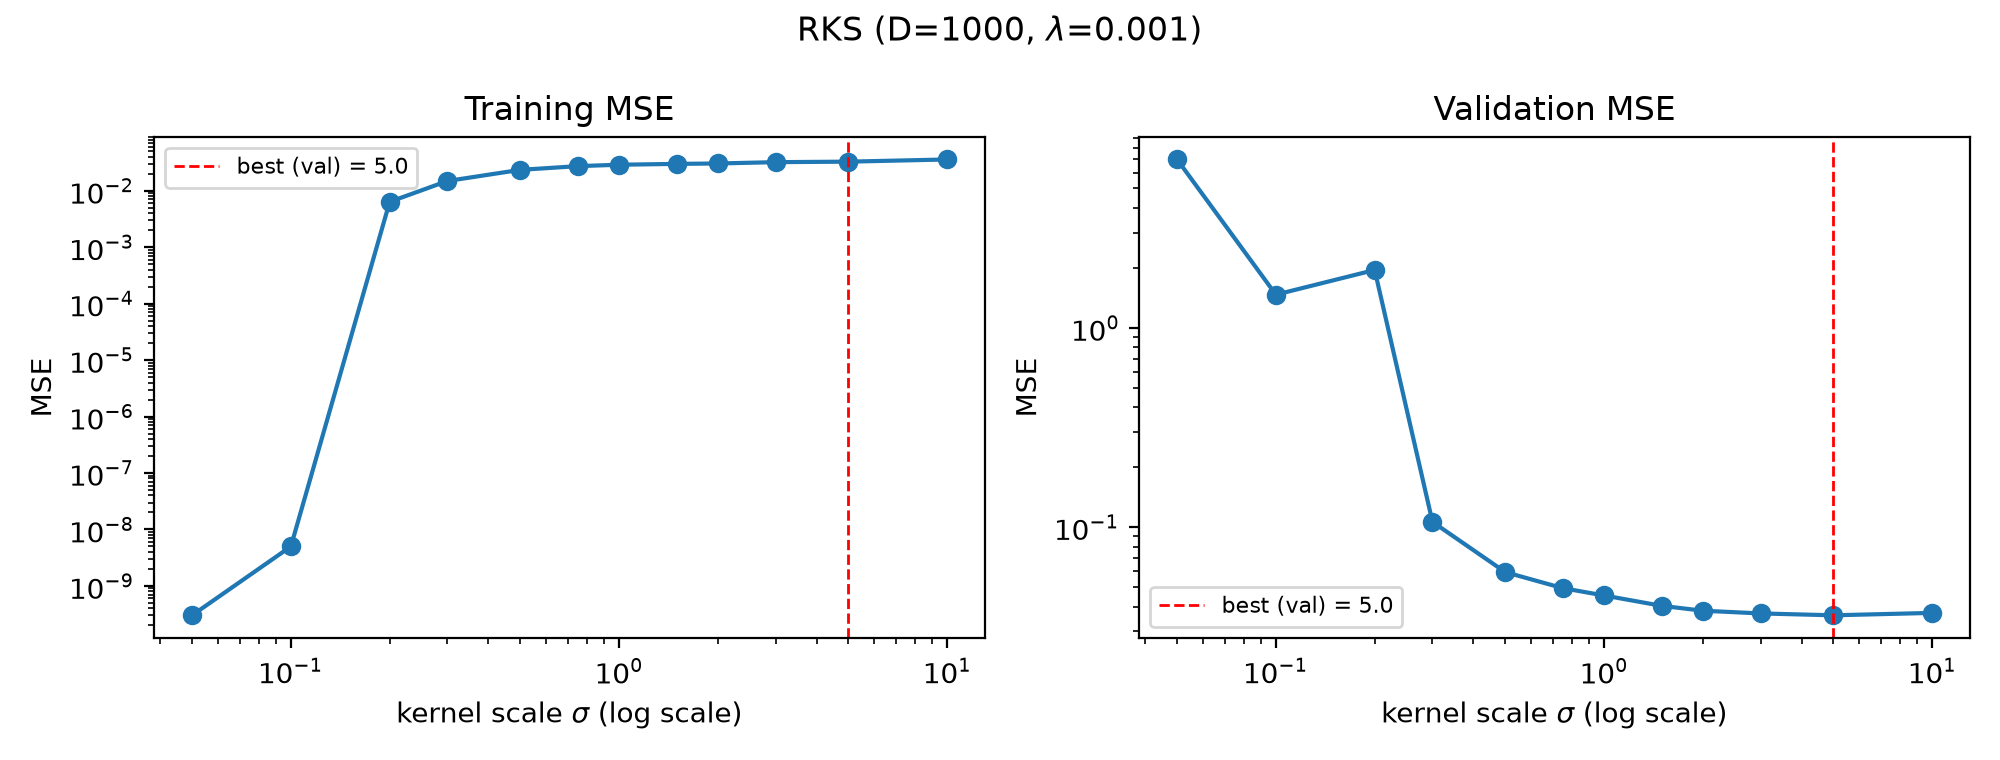
\includegraphics[width=0.95\linewidth]{../problem3/results/rks_sweep.png}
\end{figure}

\begin{table}[H]
\centering\small
\resizebox{\linewidth}{!}{\begin{tabular}{l*{12}{c}}
\toprule
$\sigma$ & 0.05 & 0.1 & 0.2 & 0.3 & 0.5 & 0.75 & 1 & 1.5 & 2 & 3 & \textbf{5} & 10 \\
\midrule
Train MSE & 0.000 & 0.000 & 0.006 & 0.015 & 0.023 & 0.027 & 0.029 & 0.030 & 0.030 & 0.032 & \textbf{0.033} & 0.036 \\
Val MSE   & 6.990 & 1.467 & 1.951 & 0.106 & 0.060 & 0.049 & 0.046 & 0.040 & 0.038 & 0.037 & \textbf{0.036} & 0.037 \\
\bottomrule
\end{tabular}}
\end{table}

\noindent A small $\sigma$ means high-frequency features: the model interpolates the training points (train MSE $\approx0$) and overfits badly. As $\sigma$ grows, the fit
becomes smoother and validation MSE drops to about 0.036. The \textbf{best value is $\sigma=5$} (validation MSE 0.0362), and at $\sigma=10$ the model starts to underfit.

\subsection*{(c)}
One-hidden-layer ReLU MLP trained with Adam (lr $3\times10^{-3}$, batch size 32, 500 epochs), sweeping the hidden width. Each width is averaged over 3 seeds.

\begin{figure}[H]
  \centering
  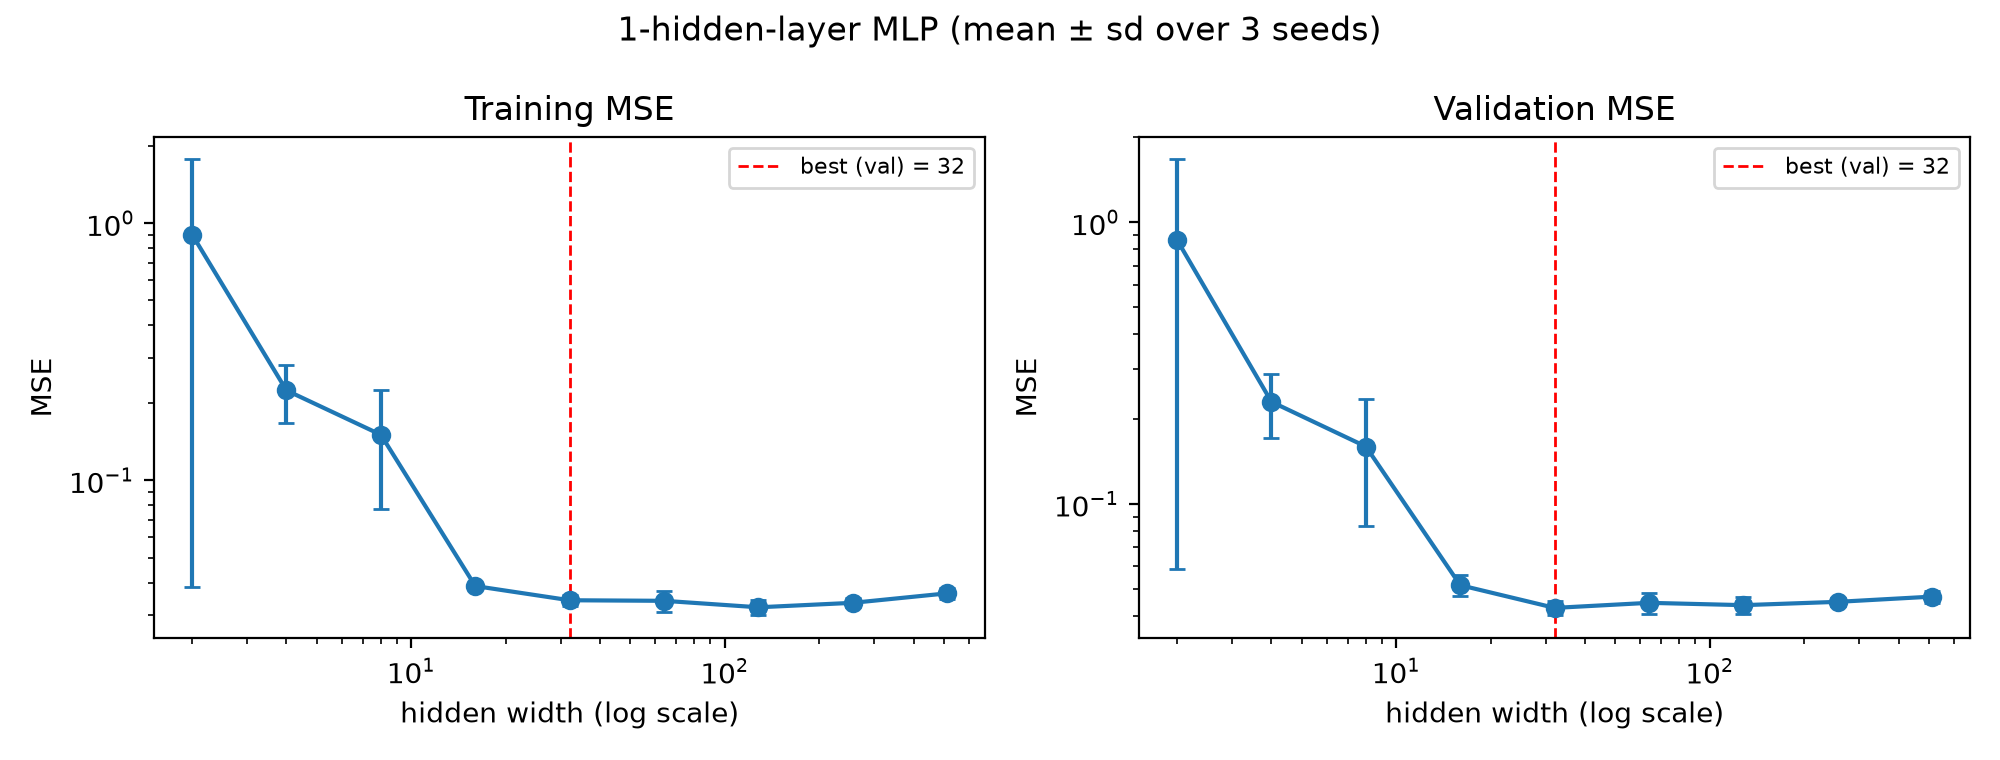
\includegraphics[width=0.95\linewidth]{../problem3/results/mlp_sweep.png}
\end{figure}

\begin{table}[H]
\centering\small
\begin{tabular}{l*{9}{c}}
\toprule
Width & 2 & 4 & 8 & 16 & \textbf{32} & 64 & 128 & 256 & 512 \\
\midrule
Train MSE & 0.902 & 0.224 & 0.150 & 0.039 & \textbf{0.034} & 0.034 & 0.032 & 0.033 & 0.036 \\
Val MSE   & 0.864 & 0.230 & 0.160 & 0.051 & \textbf{0.043} & 0.045 & 0.044 & 0.045 & 0.047 \\
\bottomrule
\end{tabular}
\end{table}

\noindent Networks with 2--8 units underfit. From 16 units on, validation MSE plateaus at about 0.043--0.047. The \textbf{best width is 32}.

\subsection*{(d)}
\begin{table}[H]
\centering\small
\begin{tabular}{lcc}
\toprule
Model & Train MSE & Validation MSE \\
\midrule
Predict training mean & -- & 2.397 \\
RKS, $\sigma=5$ & 0.0327 & \textbf{0.0362} \\
MLP, width 32 & 0.0333 & 0.0422 \\
\bottomrule
\end{tabular}
\end{table}

\begin{figure}[H]
  \centering
  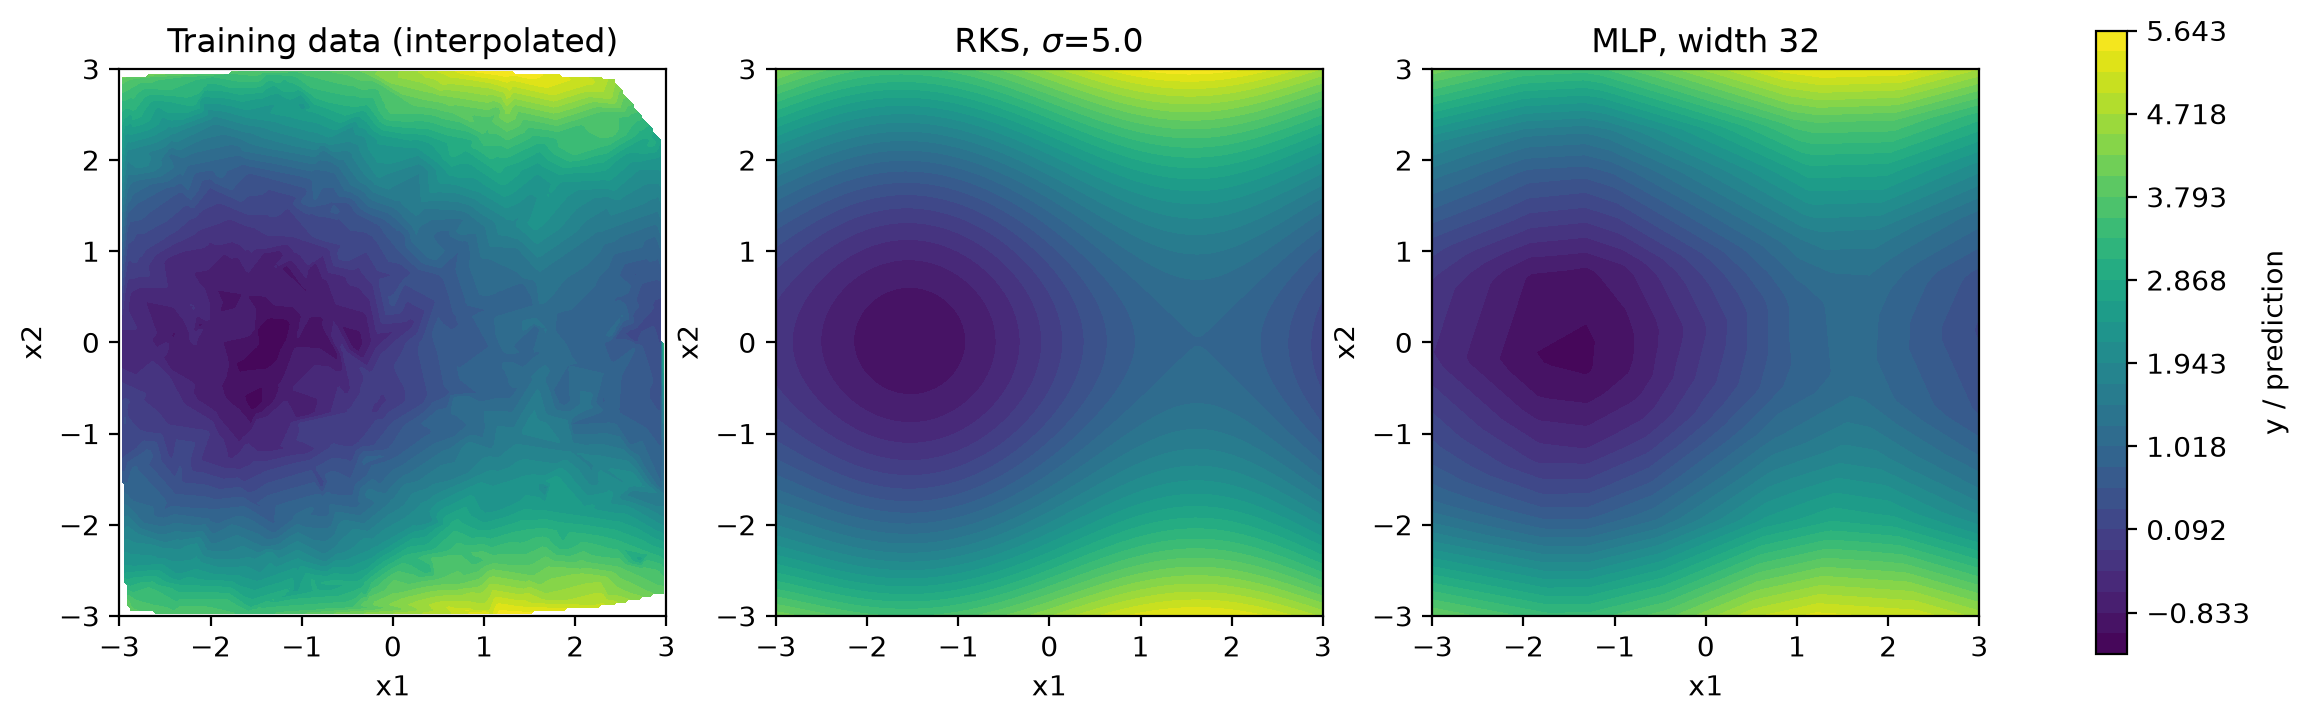
\includegraphics[width=\linewidth]{../problem3/results/surface_comparison.png}
  \caption{Interpolated training data vs.\ fitted RKS and MLP surfaces (shared color scale).}
\end{figure}

\noindent \textbf{RKS performs better} (validation MSE 0.0362 vs.\ 0.0422). Both models recover the structure seen in (a): the basin, the saddle, and the ridges at $x_2=\pm3$.
RKS approximates Gaussian-kernel ridge regression. With $\sigma=5$ all of its features are low-frequency, which builds in a smoothness assumption that matches this target,
and the fit is a convex problem solved exactly. Its surface is smooth, with round contours. The ReLU MLP is piecewise linear, so its surface is made of flat facets (visible as
polygonal contours around the basin). Approximating a curved surface this way leaves some systematic error, and its non-convex training adds seed-to-seed variance. With
only 600 points in two dimensions, learning the features gives no advantage over a well-tuned random Fourier basis.

\end{document}
